\documentclass[11pt]{article}

% TODO
% [ ] Aumentar la separación entre párrafos
% [ ] Añadir algunas bases matematicas de lo que estamos haciendo

% Paquetes
%===============================================================================

% Paquete para incluir imagenes
\usepackage{graphicx}
\graphicspath{ {./Imagenes/} }

% Paquete para incluir trozos de codigo
\usepackage{listings}


% Metadatos del documento
\title{Práctica 1 - Memoria}
\author{Sergio Quijano Rey}
\date{\today}

\begin{document}

% Portada del documento
\maketitle
\pagebreak

% Indice de contenidos
\tableofcontents
\pagebreak

% Primer ejercicio
\section{Ejercicio 1 - Búsqueda iterativa de óptimos}

% Apartado 1
\subsection{Apartado 1}

En este apartado se nos pide implementar el algoritmo de Grandiente Descendente. Esta función toma como parámetros de entrada:

\begin{itemize}
    \item \lstinline{starting_point}: punto inicial del que parte la búsqueda
    \item \lstinline{loss_function}: función de error que buscamos minimizar. En nuestro caso concreto, es una función real de dos variables
    \item \lstinline{gradient}: función vectorial 2-dimensional que representa el gradiente de \lstinline{loss_function}
    \item \lstinline{learning_rate}: la tasa de aprendizaje. Es el parámetro crítico, pues en esta sección nos centramos en estudiar el comportamiento del gradiente descendente en base a este parámetro (y también del starting\_point)
    \item \lstinline{max_iterations}: número máximo de iteraciones. Así tenemos una condición sufiente para saber que el algoritmo va a parar
    \item \lstinline{target_error}: error debajo del cual paramos de iterar
    \item \lstinline{verbose}: si es \lstinline{True}, la función devuelve el error de cada solución de las iteraciones
\end{itemize}

Esta función devuelve el vector de soluciones que hemos ido construyendo. Si queremos obtener la solución final, lo único que tenemos que hacer es acceder a la última posición. Así podemos generar las gráficas en las que plasmamos tanto la función de error como los puntos que vamos construyendo. También, si tenemos activado el parámetro Verbose, devolvemos el error en cada iteración, lo que es necesario para hacer las gráficas de evolución de error que se nos piden.

\subsection{Apartado 2}
\label{seccion:Apartado2}

Consideramos la función de error dada por:

\begin{displaymath}
    E(u, v) := (u^3 * e^{v-2} - 2v^2 e^{-u})^2
\end{displaymath}

Usar gradiente descendente para encontrar un mínimo de esta función, comenzando desde el punto $(u, v) = (1, 1)$ y
usando una tasa de aprendizaje $\eta = 0,1$.

Podemos mostrar la función de error en una vista de pájaro (la vista tridimensional solo será necesaria en casos en los que la vista de pájaro no sea suficiente). Preferimos esta vista bidimensional porque es más rápida de computar y en muchos casos más fácil de interpretar.

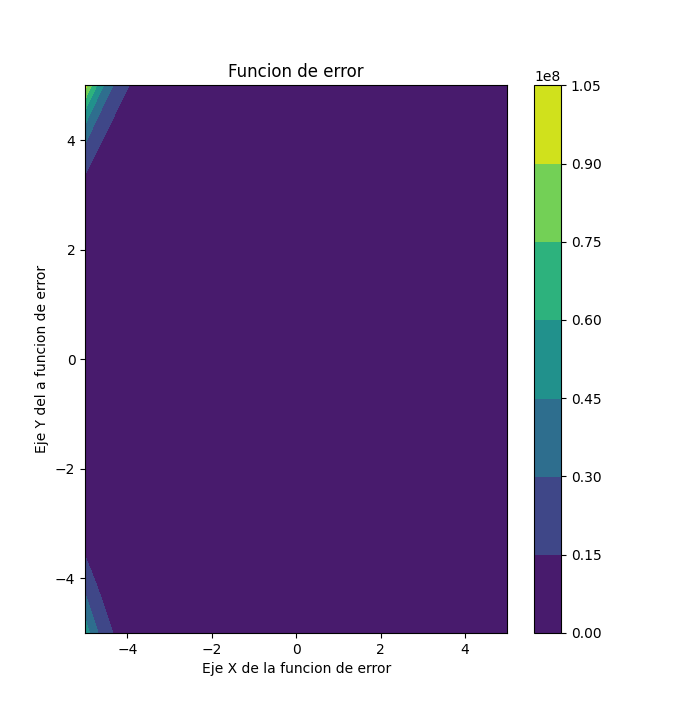
\includegraphics[scale=0.75]{FuncionErrorEjercicio1}

Los colores más azulados y oscuros indican los valores más bajos del error, mientras que valores verdosos y claros indican valores altos del error (la leyenda de la gráfica ya indica esto). Así que nuestros puntos deberán ir acercándose a zonas oscuras de la gráfica, si el comportamiento de los algoritmos es bueno.


\subsubsection{Subapartado a}

Calculamos analíticamente la expresión de las derivadas parciales:

\begin{displaymath}
    \frac{\partial E}{\partial u} = 2 * (u^3 * e^{v-2} - 2v^2 e^{-u}) * (3u^2 e^{v-2} + 2v^2 e^{-u}) \\
\end{displaymath}
\begin{displaymath}
    \frac{\partial E}{\partial v} = 2 * (u^3 * e^{v-2} - 2v^2 e^{-u}) * (u^3 * e^{v-2} - 4v e^{-u})  \\
\end{displaymath}
\begin{displaymath}
    \nabla E = (\frac{\partial E}{\partial u}, \frac{\partial E}{\partial v})
\end{displaymath}

Esta es la expresión del gradiente que usamos en el código. Expresión que mostramos por pantalla, como se indica en el guión de la práctica.

\subsubsection{Subapartados b y c}

Se manda explícitamente que usemos flotantes de 64 bits, para lo cual usamos la orden \lstinline{np.float64} para devolver todas nuestras funciones que representan los errores y las derivadas parciales.

Como se muestra en el código, solo necesitamos 10 iteraciones para quedarnos por debajo de un error (o valor de $E(u, v)$, que es lo que estamos considerando como función de error a minimizar) de valor $10^{-14}$. En el código indicamos que la primera iteración por debajo del error es la iteración 9, pero hay que tener en cuenta que empezamos a contar desde el cero.

Los resultados que mostramos por pantalla nos indican que alcanzamos la solución:

\begin{verbatim}
Numero de iteraciones: 10
Pesos encontrados: [1.15728885 0.91083837]
\end{verbatim}

Estos son los resultados vinculados a la onceava iteración (recordar que empezamos a contar desde el cero). Los resultados asociados a la décima iteración, en los que ya estamos por debajo del error buscado, son:

\begin{verbatim}
Primera iteracion por debajo de 10e-14: 9 (contando desde cero)
Las primeras coordenadas por debajo del error: [1.15728875 0.9108384 ]
\end{verbatim}

Todo esto se muestra en las salidas por pantalla de nuestro programa. Además, podemos mostrar cómo avanzan nuestras soluciones sobre la superficie que representa la función de error:

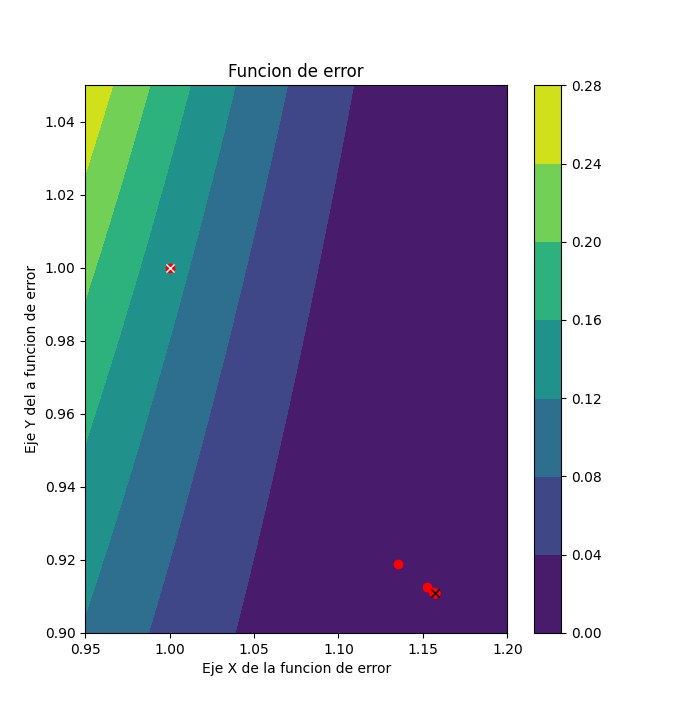
\includegraphics[scale=0.75]{EvolucionSoluciones01}

El punto con una cruz blanca es el punto inicial. El punto con una cruz negra es el punto final de la búsqueda. Viendo la gráfica de las soluciones generadas es claro que podríamos seguir avanzando con la búsqueda, pero decidimos parar porque estamos por debajo de la cota de error pedida.

La gráfica del error para los parámetros que se nos han indicado en ~\ref{seccion:Apartado2} es la siguiente:

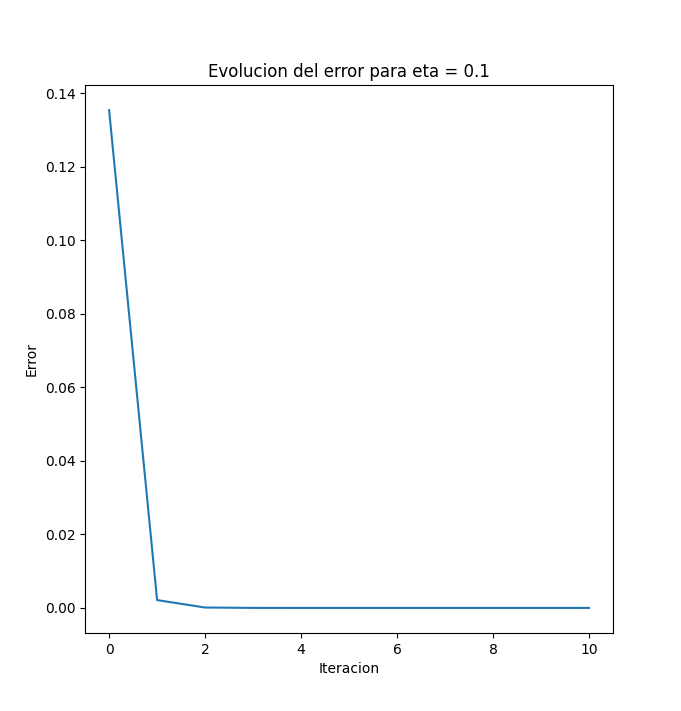
\includegraphics[scale=0.75]{EvolucionError01}

\subsection{Apartado 3}

Se considera ahora la función:

\begin{displaymath}
    f(x,y) := (x+2)^2 + 2(y-2)^2 + 2 sin(2\pi x) sin(2 \pi y)
\end{displaymath}

Como vamos a usar la técnica del gradiente descendente, necesitamos calcular analíticamente la expresión del gradiente:

\begin{displaymath}
    \frac{\partial f(x,y)}{\partial x} = 2(x+2) + 4 \pi sin(2 \pi y) cos(2 \pi x)
\end{displaymath}
\begin{displaymath}
    \frac{\partial f(x,y)}{\partial y} = 4(y - 2) + 4 \pi sin(2 \pi x) cos(2 \pi y)
\end{displaymath}
\begin{displaymath}
    \nabla f(x, y) = (\frac{\partial f(x,y)}{\partial x}, \frac{\partial f(x,y)}{\partial y})
\end{displaymath}

\subsubsection{Apartado a}

Se nos pide usar gradiente descendiente para minimizar la función de error $f$. Además, se nos pide que usemos como parámetros del gradiente descendente:

\begin{itemize}
    \item $\eta = 0.01$
    \item $x_0 = -1, y_0 = 1$
    \item Máximo 50 iteraciones
\end{itemize}

Y que repitamos el experimento con un valor de $\eta = 0.1$.

Lo primero que hacemos es mostrar una gráfica en dos dimensiones de la función de error que queremos minimizar:

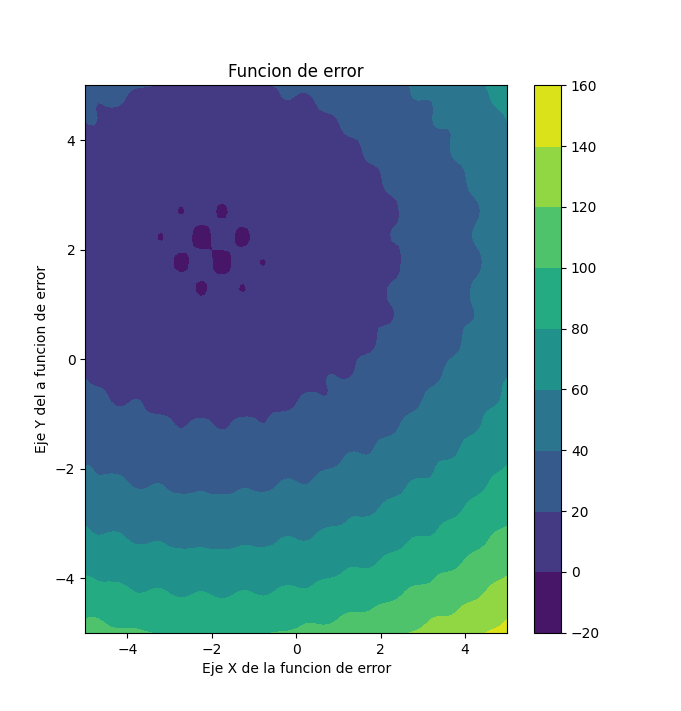
\includegraphics[scale=0.65]{FuncionErrorEjercicio1Apartado3}

Realizando gradiente descendente con los primeros parametros dados obtenemos la siguiente gráfica, en la que se muestra cómo evoluciona el valor del error según avanzan las iteraciones del algoritmo.

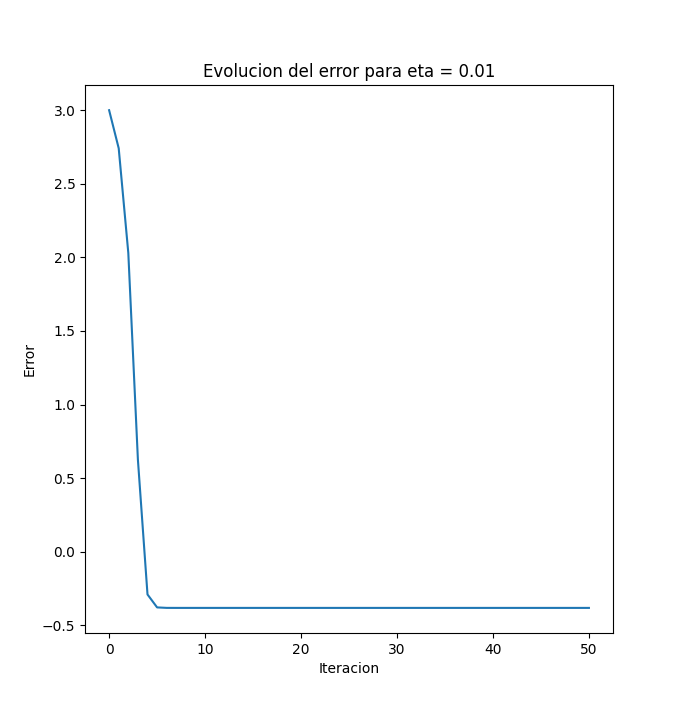
\includegraphics[scale=0.65]{EvolucionError02}

Mostramos, aunque no se nos pida en el guión, la traza del algritmo (soluciones plasmadas sobre la gráfica bidimensiona del error):

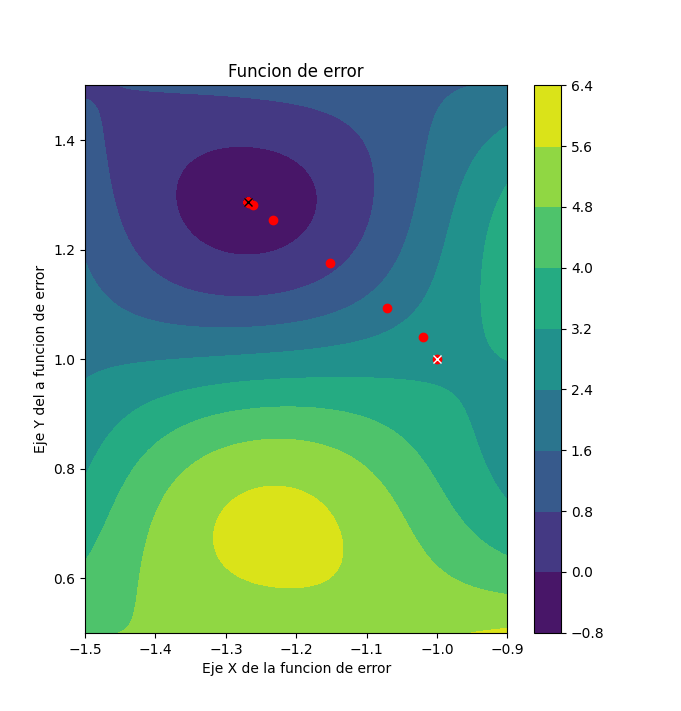
\includegraphics[scale=0.65]{EvolucionSoluciones02}

En esta gráfica se puede apreciar con facilidad que el algoritmo tiene el comportamiento deseado, pues cae con facilidad en un óptimo local.

Ahora realizamos el mismo proceso pero cambiando a $\eta = 0.1$. Obtenemos la siguiente gráfica de evolución del errolución del error:

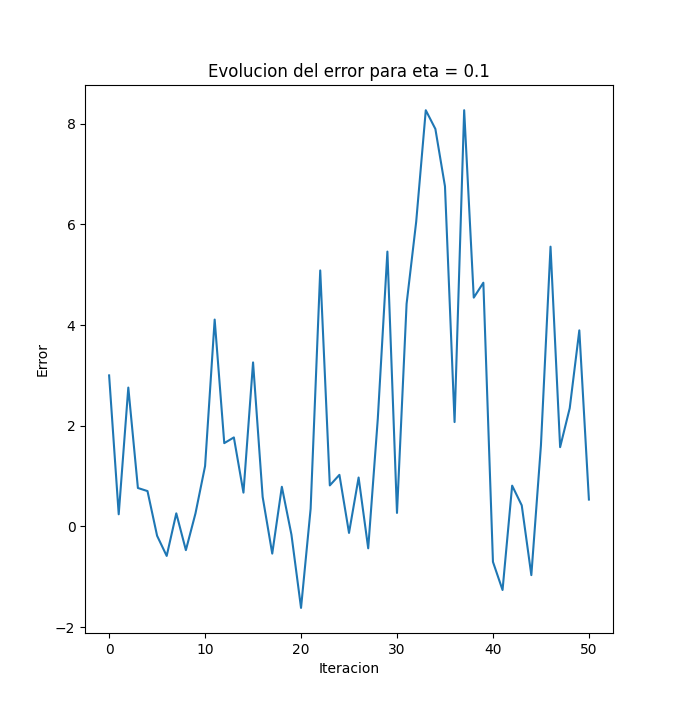
\includegraphics[scale=0.65]{EvolucionError03}

De esta gráfica ya podemos ver que el comportamiento del algoritmo no es el deseado. Lo que esperaríamos es que el error disminuyese monótamente en cada iteración. Sin embargo, lo que nos encontramos es con que el error oscila con grandes saltos. De lo estudiado en teoría, sabemos que el motivo sea seguramente un valor de $\eta$ demasiado grande. COn esto, cuando estamos cerca de una solución local, damos un salto muy grande en cierta dirección, saltando el óptimo local y yendo a una zona de alto error. Del mismo modo, de un salto desde una zona de alto error podemos acabar en una zona de muy bajo error. Es claro que este comportamiento errático no es deseable. Mostramos la traza de las soluciones en cada iteración para reforzar esta hipótesis sobre el mal comportamiento:

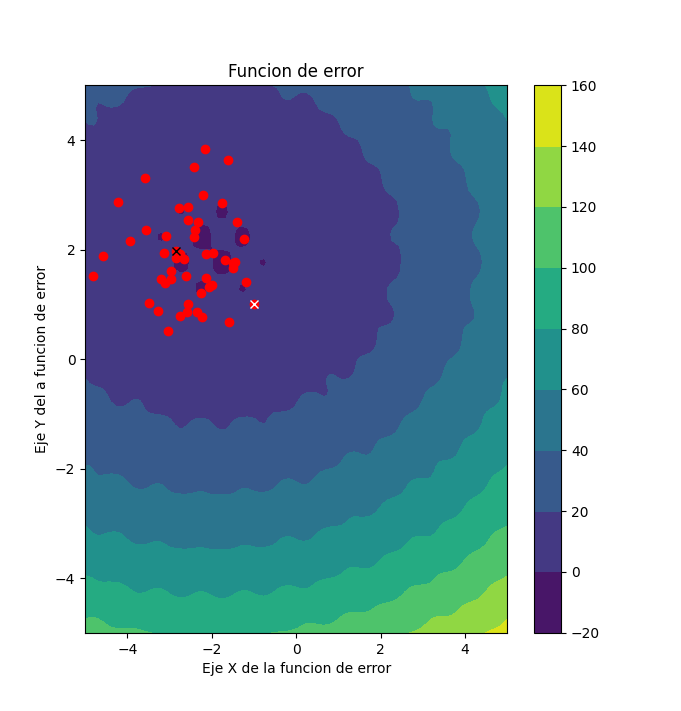
\includegraphics[scale=0.65]{EvolucionSoluciones03}

Con este gráfico, vemos que en la última iteración (del gráfico de evolución de error se deduce ya que se han consumido el total de iteraciones) hemos acabado, por buena suerte, en una buena zona de la función del error.

Con este ejemplo, podemos ver que es importante explorar con distintos valores de $\eta$, pues estos influyen mucho en el buen o mal comportamento del gradiente descendiente. Es más, ya podemos intuir que un ajuste dinámico del valor de $\eta$ puede ser muy interesante, pues como hemos visto en teoría, nos interesa avanzar con \emph{"pasos de gigante"} al principio con un $\eta$ grande, y disminuir el valor de $\eta$ al acercarnos a un óptimo local para tener más precisión en las iteraciones.

En estos dos ejemplos no muestro los valores numéricos de las soluciones obtenidas ni del error alcanzado. Considero que es mucho más interesante e informativo visualizar las gráficas, tanto del error como de la traza, pues estamos estudiando el comportamiento del algoritmo, no una solución concreta que no nos interesa al no ser un problema que realmente queramos resolver.

\subsubsection{Apartado b}

\end{document}
